\subsection{Target of inference: the pool or the population}\label{sec:population}

The intervals of Section~\ref{sec:design} cover the contrast computed on the pool, $\theta_U=f(T_U)$. If the pool is itself a sample of $N$ units from a deployment population, the quantity of interest is the population contrast $\theta_{\rm pop}=\tilde f(\tau)$, $\tau=\mathrm E\,t_i(Y_i)$, and the pool-conditional interval ignores the pool's sampling error. Write $\hat\theta=f(T_{\rm dif})$ for the unchanged estimator. Then
\[
\hat\theta-\theta_{\rm pop}=\underbrace{f(T_{\rm dif})-f(T_U)}_{\text{design error}}+\underbrace{f(T_U)-f(N\tau)}_{\text{pool error}} .
\]
Given the pool, the first term has mean zero to first order and variance $V_{\rm design}=\sum_h N_h^2(1-n_h/N_h)S_h^2(e)/n_h$, the quantity estimated in Section~\ref{sec:design}. The second term is, to first order, a sum of $N$ independent influence values, so the two terms are uncorrelated and
\begin{equation}\label{eq:pop-variance}
\begin{gathered}
V_{\rm total}=\mathrm E\,V_{\rm design}+V_{\rm pool},\\
V_{\rm pool}=N\,\mathrm{Var}(z_i),\qquad z_i=\mathbf b^{\top}\bigl(t_i(Y_i)-\tau\bigr),
\end{gathered}
\end{equation}
with $\mathbf b=\nabla f(N\tau)$ the gradient on the scale of totals. This is the two-phase decomposition of \citet{sarndal1987}. The influence value $z_i$ is that of the full-label plug-in contrast, not the residual $e_i$ of the difference estimator: the proxy removes variance from the labelled part of the error but cannot remove the variation of $Y$ across units of the population, so, to first order, $V_{\rm pool}$ is the same for every labelling design and every proxy.

Since the labelled sample is a stratified sample of the pool, $V_{\rm pool}$ is estimated with the weights $w_i=N_h/n_h$:
\[
\begin{gathered}
\hat V_{\rm pool}=\sum_{i\in s}w_i\,(\hat z_i-\bar z)^2,\\
\bar z=\frac1N\sum_{i\in s}w_i\hat z_i,\qquad \hat z_i=\hat{\mathbf b}^{\top}t_i(Y_i),
\end{gathered}
\]
with $\hat{\mathbf b}=\nabla f(T_{\rm dif})$, and the two-phase interval is $\hat\theta\pm1.96\sqrt{\hat V_{\rm design}+\hat V_{\rm pool}}$. The derivation is in \texttt{docs/two\_phase\_note.md} and the code in \texttt{tcs/labeling\_two\_phase.py}. Let $\varpi=V_{\rm pool}/V_{\rm design}$. It is of order $L\,\mathrm{Eff}/N$, where $\mathrm{Eff}$ is the efficiency of the design against SRS, so it grows with the budget and the efficiency and shrinks with the pool size. With correct $V_{\rm design}$ and normal errors the pool-conditional interval has coverage about $2\Phi(1.96/\sqrt{1+\varpi})-1$ of the population contrast, which is $0.93$ at $\varpi=0.2$, $0.83$ at $\varpi=1$ and $0.67$ at $\varpi=3$. Efficiency changes in the same way: the pool term is shared by SRS and PATTERN-DIF, so against the population contrast the MSE ratio is $(\mathrm{Eff}+\varpi)/(1+\varpi)$, with $\varpi$ evaluated for PATTERN-DIF, rather than $\mathrm{Eff}$. For $\mathrm{Eff}=6$ and $\varpi=1.5$ this is $3$. This follows arithmetically from \eqref{eq:pop-variance}; it is not an estimate from the earlier experiments.

\subsubsection*{Experiment}
We checked the two intervals against population values in a synthetic setting; the real data sets are not used. The population is the generative model of the non-smooth simulation (five Gaussian covariates, a group with prevalence $0.3$, a logistic label model) with nine fixed scoring rules, so there are $36$ pairs and $108$ contrasts, $\theta^{TPR}$, $\theta^{FPR}$ and $\theta^{ERR}$. Population values were computed on $6\times10^{6}$ draws. For every replicate a new pool of $N\in\{2000,8000,20000\}$ units is drawn and then a PATTERN-DIF sample (PATTERN strata, plain allocation, difference estimator) of $L\in\{250,500,1000,2000\}$ labels ($L\le N/4$; ten cells), with the mean-probability proxy; $R=300$ replicates per cell. Table~\ref{tab:pop-check} and Figure~\ref{fig:pop-check} give the coverage, averaged over the $108$ contrasts and for the worst contrast, together with the median over contrasts of $\hat V_{\rm pool}/\hat V_{\rm design}$ (source: \texttt{results/two\_phase\_check.json}).

\begin{table}[t]
\centering\small
\caption{Coverage of the population contrast (nominal $0.95$) over $108$ contrasts, $R=300$ pools per row. $V_{\rm pool}/V_{\rm des}$ is the median over contrasts of the estimated ratio. The last column is the coverage of the pool value by the pool-conditional interval. Source: \texttt{results/two\_phase\_check.json}.}\label{tab:pop-check}
\begin{tabular}{rr r rr rr r}\toprule
 & & & \multicolumn{2}{c}{Pool-conditional} & \multicolumn{2}{c}{Two-phase} & Pool value \\
$N$ & $L$ & $V_{\mathrm{pool}}/V_{\mathrm{des}}$ & mean & worst & mean & worst & (pool-cond.) mean \\\midrule
2{,}000 & 250 & 0.50 & 0.899 & 0.86 & 0.949 & 0.92 & 0.949 \\
 & 500 & 1.51 & 0.809 & 0.72 & 0.952 & 0.92 & 0.948 \\
\addlinespace
8{,}000 & 250 & 0.11 & 0.940 & 0.91 & 0.951 & 0.92 & 0.952 \\
 & 500 & 0.25 & 0.921 & 0.87 & 0.947 & 0.90 & 0.948 \\
 & 1000 & 0.58 & 0.889 & 0.83 & 0.950 & 0.92 & 0.945 \\
 & 2000 & 1.57 & 0.792 & 0.64 & 0.949 & 0.92 & 0.953 \\
\addlinespace
20{,}000 & 250 & 0.04 & 0.940 & 0.90 & 0.945 & 0.91 & 0.945 \\
 & 500 & 0.09 & 0.942 & 0.90 & 0.952 & 0.91 & 0.953 \\
 & 1000 & 0.20 & 0.928 & 0.89 & 0.947 & 0.92 & 0.949 \\
 & 2000 & 0.44 & 0.903 & 0.83 & 0.949 & 0.91 & 0.949 \\
\bottomrule\end{tabular}

\end{table}

\begin{figure}[t]
\centering
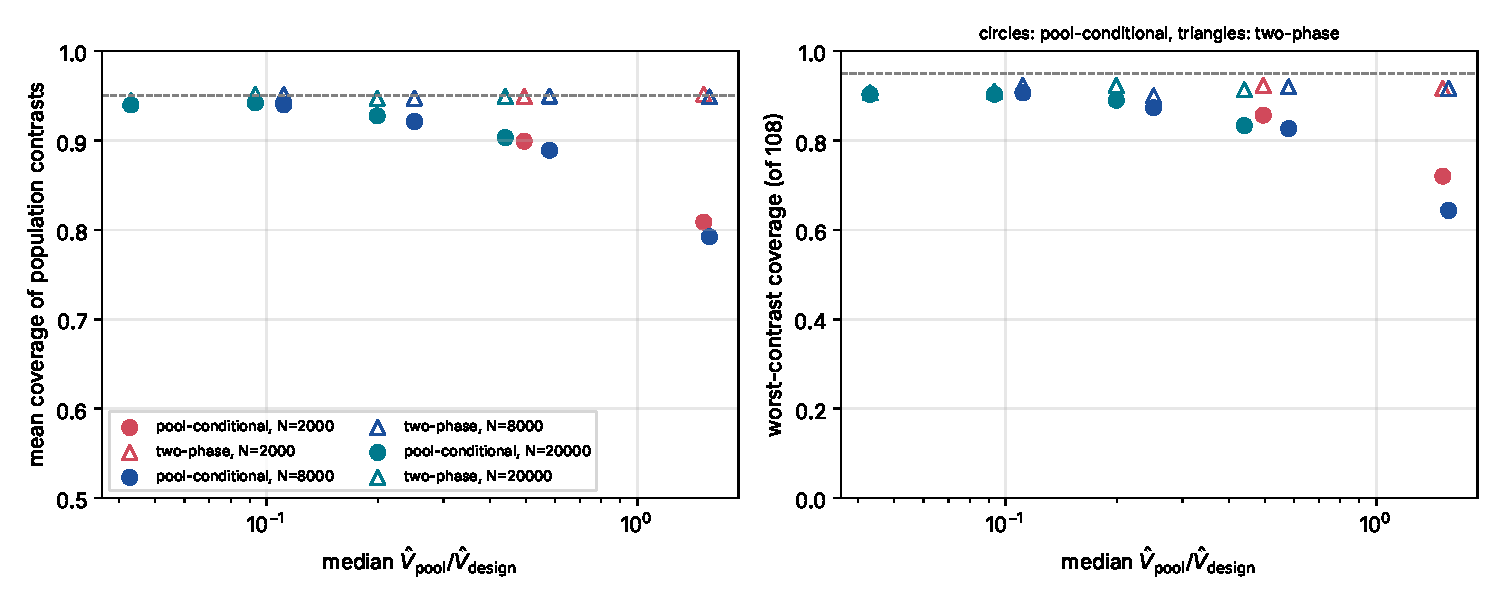
\includegraphics[width=\textwidth]{figures/two_phase_check}
\caption{Coverage of the population contrasts against the median ratio $\hat V_{\rm pool}/\hat V_{\rm design}$, one point per $(N,L)$ cell. Left: mean over the $108$ contrasts. Right: worst contrast. Circles: pool-conditional intervals, triangles: two-phase intervals; colours give $N$.}\label{fig:pop-check}
\end{figure}

The pool-conditional interval keeps its coverage of the pool value (mean $0.945$ to $0.953$ in all ten cells), so the earlier results are not affected. Against the population contrast its mean coverage falls with $\varpi$: $0.94$ when $\varpi\le0.11$, $0.90$ to $0.93$ for $\varpi$ between $0.2$ and $0.5$, $0.89$ at $\varpi=0.58$ and $0.79$ to $0.81$ at $\varpi\approx1.5$ (the cells $N=2000,L=500$ and $N=8000,L=2000$), where the worst contrast is covered in $0.72$ and $0.64$ of the replicates. This is close to the value the formula predicts. The two-phase interval has mean coverage $0.945$ to $0.952$ in every cell and worst-contrast coverage $0.90$ to $0.92$. The worst of $108$ contrasts with $300$ replicates has a Monte Carlo standard error of $0.013$, so the worst value is expected to lie near $0.92$ even for exact intervals. We do not read the remaining gap as a failure, but the experiment cannot exclude a small one. The cost is width: the two-phase interval is $2\%$ to $10\%$ wider when $\varpi\le0.2$, $12\%$ wider at $\varpi=0.25$ and $21\%$ to $71\%$ wider when $\varpi\ge0.44$ (median width over contrasts).

\subsubsection*{When the pool term matters}
It does not matter when $N$ is large relative to the budget: at $N=20000$ and $L\le500$, $\varpi\le0.09$ and the two intervals are nearly the same. It matters when the labelled fraction is not small, as in the small pools of the empirical study (about $2000$ to $20000$ instances, budgets up to $2000$). The empirical MSE of $\hat\theta$ around the population contrast is $1.04$ to $2.6$ times its MSE around the pool contrast in these cells. Three limits apply. The simulation is stylised: the pool is an independent sample of the population and the models are fixed and independent of the pool. With real data the deployment population is unknown, the pool may be a convenience sample, and the two-phase interval is only as good as the assumption that the pool is representative. If the pool is the whole deployment set, the pool-conditional interval is the right one and the two-phase interval is conservative. The gain of PATTERN-DIF over SRS also shrinks for the population target, as shown above, although the ranking of designs does not change. We did not run the full pipeline (training, pooling, labelling) against full-data references on the OpenML data; the known population above isolates the pool-sampling term.
